%%%%%%%%%%%%%%%%%%%%%%%%%%%%%%%%%%%%%%%%% 
% Beamer Presentation LaTeX Template Version 1.0 (10/11/12)
% 
% This template has been downloaded from:
% http://www.LaTeXTemplates.com
% 
% License: CC BY-NC-SA 3.0
% (http://creativecommons.org/licenses/by-nc-sa/3.0/)
% 
%%%%%%%%%%%%%%%%%%%%%%%%%%%%%%%%%%%%%%%%% 

% ----------------------------------------------------------------------------------------
% PACKAGES AND THEMES
% ----------------------------------------------------------------------------------------

\documentclass{beamer}

\mode<presentation> {

  % The Beamer class comes with a number of default slide themes
  % which change the colors and layouts of slides. Below this is a
  % list
  % of all the themes, uncomment each in turn to see what they look
  % like.

  % \usetheme{default}
  % \usetheme{AnnArbor}
  % \usetheme{Antibes}
  % \usetheme{Bergen}
  % \usetheme{Berkeley}
  % \usetheme{Berlin}
  % \usetheme{Boadilla}
  % \usetheme{CambridgeUS}
  % \usetheme{Copenhagen}
  % \usetheme{Darmstadt}
  % \usetheme{Dresden}
  % \usetheme{Frankfurt}
  \usetheme{Goettingen}
  % \usetheme{Hannover}
  % \usetheme{Ilmenau}
  % \usetheme{JuanLesPins}
  % \usetheme{Luebeck}
  % \usetheme{Madrid}
  % \usetheme{Malmoe}
  % \usetheme{Marburg}
  % \usetheme{Montpellier}
  % \usetheme{PaloAlto}
  % \usetheme{Pittsburgh}
  % \usetheme{Rochester}
  % \usetheme{Singapore}
  % \usetheme{Szeged}
  % \usetheme{Warsaw}

  % As well as themes, the Beamer class has a number of color themes
  % for any slide theme. Uncomment each of these in turn to see how it
  % changes the colors of your current slide theme.

  % \usecolortheme{albatross}
  % \usecolortheme{beaver}
  % \usecolortheme{beetle}
  % \usecolortheme{crane}
  % \usecolortheme{dolphin}
  % \usecolortheme{dove}
  % \usecolortheme{fly}
  % \usecolortheme{lily}
  % \usecolortheme{orchid}
  % \usecolortheme{rose}
  % \usecolortheme{seagull}
  % \usecolortheme{seahorse}
  % \usecolortheme{whale}
  % \usecolortheme{wolverine}

  % \setbeamertemplate{footline} % To remove the footer line in all slides uncomment this line
  \setbeamertemplate{footline}[page
  number] % To replace the footer line in all slides with a simple slide count uncomment this line

  % \setbeamertemplate{navigation
  % symbols}{} % To remove the navigation symbols from the bottom of all slides uncomment this line
}

\usepackage{graphicx} % Allows including images
\usepackage{booktabs} % Allows the use of \toprule, \midrule and \bottomrule in tables
\usepackage[german]{babel} % Required to compile in Windows
\usepackage[utf8]{inputenc}
% \usepackage{physics}
\usepackage{mathtools}
\usepackage{natbib}
\usepackage[T1]{fontenc}


\AtBeginSection[]{
  \begin{frame}
    \vfill \centering
    \begin{beamercolorbox}[sep = 8pt, center, shadow = true, rounded =
      true]{title}
      \usebeamerfont{title}\insertsectionhead\par%
    \end{beamercolorbox}
    \vfill
  \end{frame}
}

% ----------------------------------------------------------------------------------------
% TITLE PAGE
% ----------------------------------------------------------------------------------------

\title[]{Projekt 1a:
  Abschlusspräsentation} % The short title appears at the bottom of every slide, the full title is only on the title page

\author{Isabell Albrecht, Erik Engelhardt, Oliver Kochan, Florian
  Steffens} % Your name
\institute[HAW] % Your institution as it will appear on the bottom of every slide, may be shorthand to save space
{ Hochschule für angewandte Wissenschaften -- Hamburg
  \\ % Your institution for the title page
  \medskip
  % \textit{erik.engelhardt@haw-hamburg.de,
  % hier@email.eintragen} % Your email address
}

\date{14. Januar 2020} % Date, can be changed to a custom date

\begin{document}

\begin{frame}
  \titlepage % Print the title page as the first slide
\end{frame}

\section{Einleitung}
% - Gruppenmitglieder vorstellen - welches Projekt bearbeiten wir
% (Bild)
\begin{frame}
  \frametitle{Wetterstation - Projekt 1a}
  \begin{figure}
    \centering
    \begin{minipage}[t]{0.45\linewidth}
      \centering
      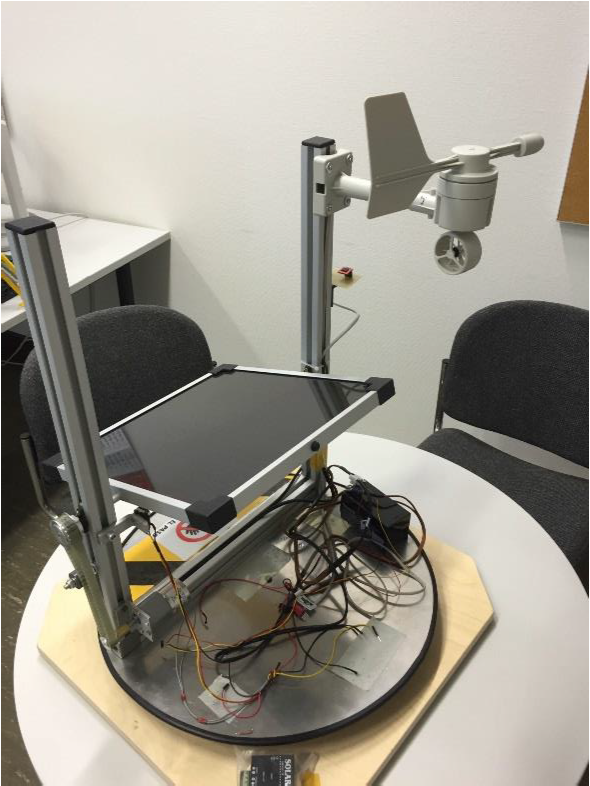
\includegraphics[width=\linewidth]{img/Wetterstation_1.png}
    \end{minipage}% <- sonst wird hier ein Leerzeichen eingefÃŒgt
    \hfill
    \begin{minipage}[t]{0.45\linewidth}
      \centering
      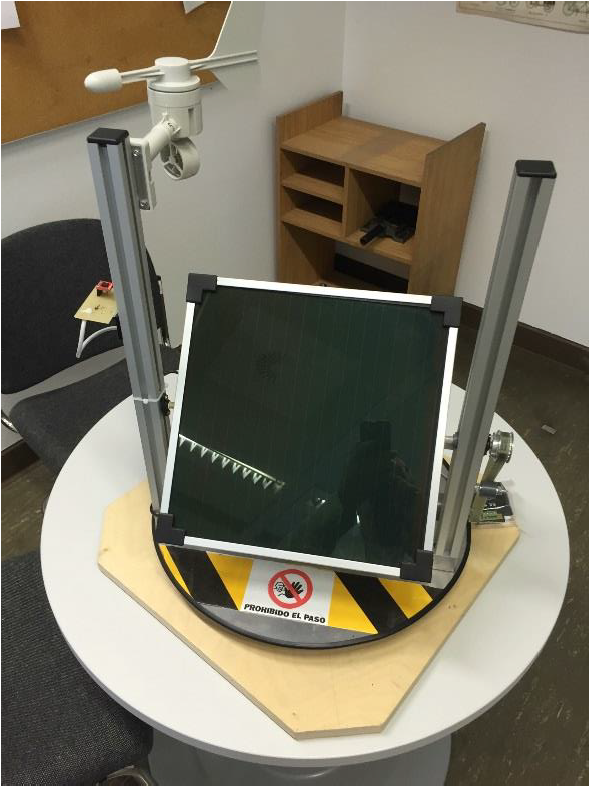
\includegraphics[width=\linewidth]{img/Wetterstation_2.png}
    \end{minipage}
  \end{figure}
  % \emph{Diese Wetterstation wird sehr gut.}
\end{frame}

\begin{frame}[allowframebreaks]
  % \frametitle{Gliederung} % Table of contents slide, comment this block out to remove it
  \tableofcontents % Throughout your presentation, if you choose to use \section{} and \subsection{} commands, these will automatically be printed on this slide as an overview of your presentation
\end{frame}
% ----------------------------------------------------------------------------------------
% PRESENTATION SLIDES NEW
% ----------------------------------------------------------------------------------------

\section{Live-Demo}

\section{Firmware}

\begin{frame}{Firmware}{Nachführung des Solarpanels}
    \begin{itemize}[<+->]
        \item Optimierung des Wirkungsgrades durch Nachführung des Panels
        \begin{itemize}
            \item Sonnenstand über Aufstellungsort und aktuellen Zeitstempel
        \end{itemize}
        \item Lageregelung unabhängig von der Aufstellungsrichtung
        \item Magnetometer: lokale Störungen kompensiert
        \item GPS-Ortung und -Zeitsynchronisation
        \begin{itemize}
            \item Auch über Bluetooth konfigurierbar
        \end{itemize}
    \end{itemize}
\end{frame}

\begin{frame}{Firmware}{Kommunikation}
    \begin{itemize}[<+->]
        \item Kommunikation nutzt AT-Protokoll
        \begin{itemize}
            \item Für Terminaleingabe und Programmverarbeitung geeignet
        \end{itemize}
        \item Serial-over-Bluetooth: Virtueller COM-Port
        \item Keine speziellen Treiber notwendig
    \end{itemize}    
\end{frame}

\begin{frame}{Firmware}{Sensordaten}
    \begin{figure}
        \centering
        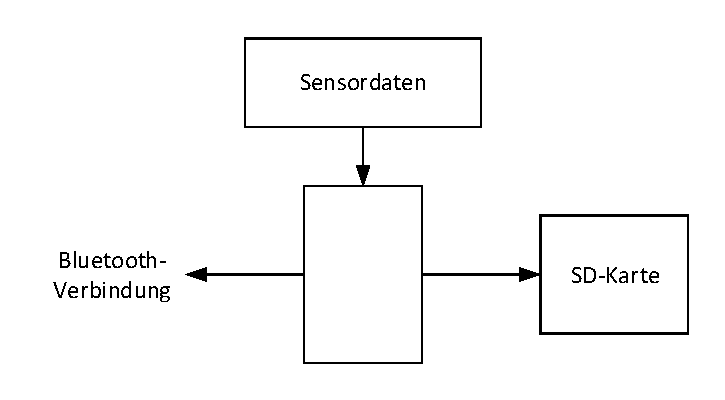
\includegraphics[width=\textwidth]{./img/Datenverteilung.pdf}
    \end{figure}
\end{frame}

\begin{frame}{Firmware}{Statusanzeige}
    \textbf{Systemstatus:}
    \begin{figure}[H]
        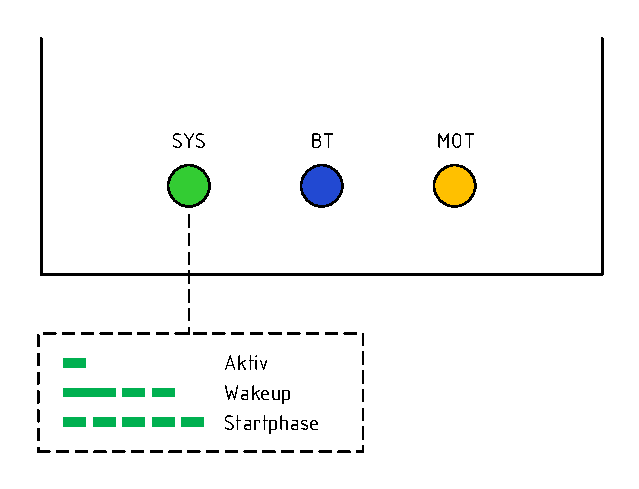
\includegraphics[width=.8\textwidth]{./img/Systemstatus.pdf}
    \end{figure}
\end{frame}

\begin{frame}{Firmware}{Statusanzeige}
    \textbf{Bluetooth Status:}
    \begin{figure}[H]
        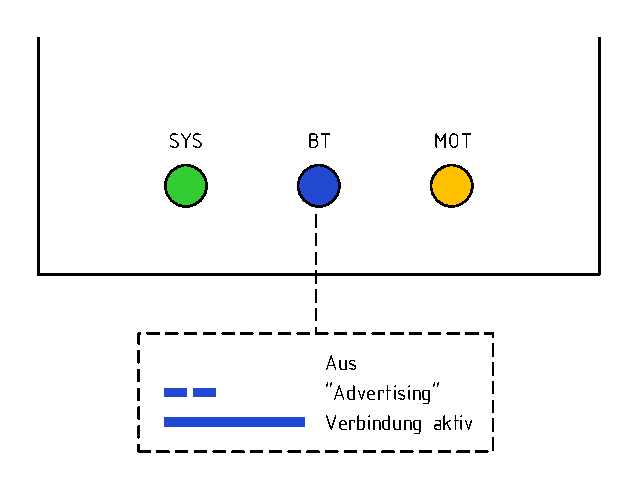
\includegraphics[width=.8\textwidth]{./img/Bluetoothstatus.pdf}
    \end{figure}
\end{frame}

\begin{frame}{Firmware}{Statusanzeige}
    \textbf{Motorsteuerung Status:}
    \begin{figure}[H]
        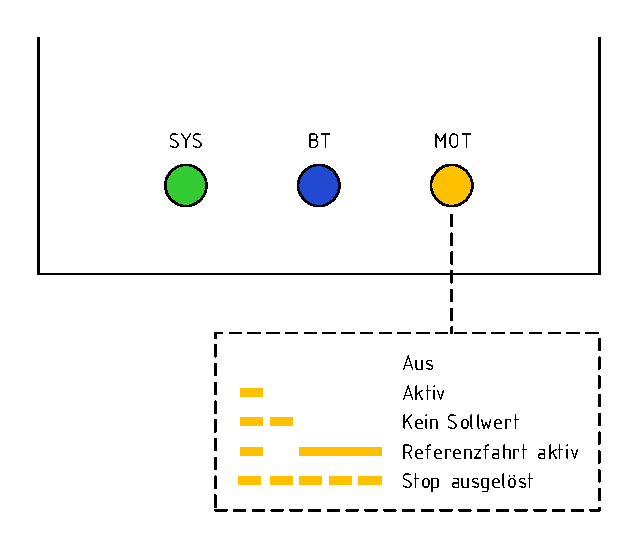
\includegraphics[width=.8\textwidth]{./img/Motorstatus.pdf}
    \end{figure}
\end{frame}

\section{Nutzeroberfläche}

\begin{frame}
  \frametitle{Funktionen}
  \begin{figure}[H]
    \centering
    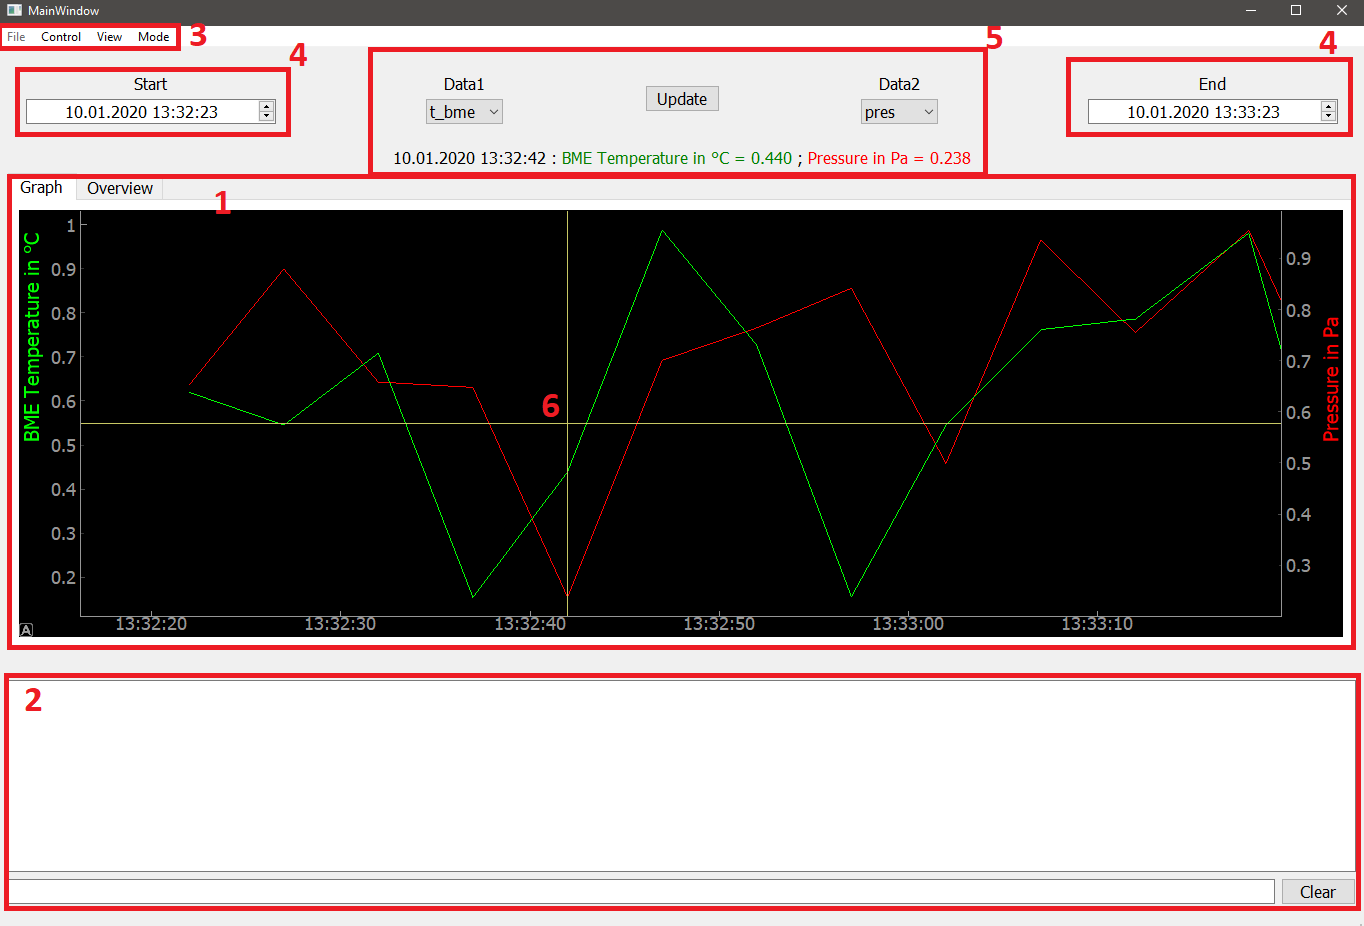
\includegraphics[width=\textwidth]{./img/ui_simulated_graph}
  \end{figure}
\end{frame}
\begin{frame}
  \frametitle{Funktionen}
  \begin{figure}[H]
  \centering
  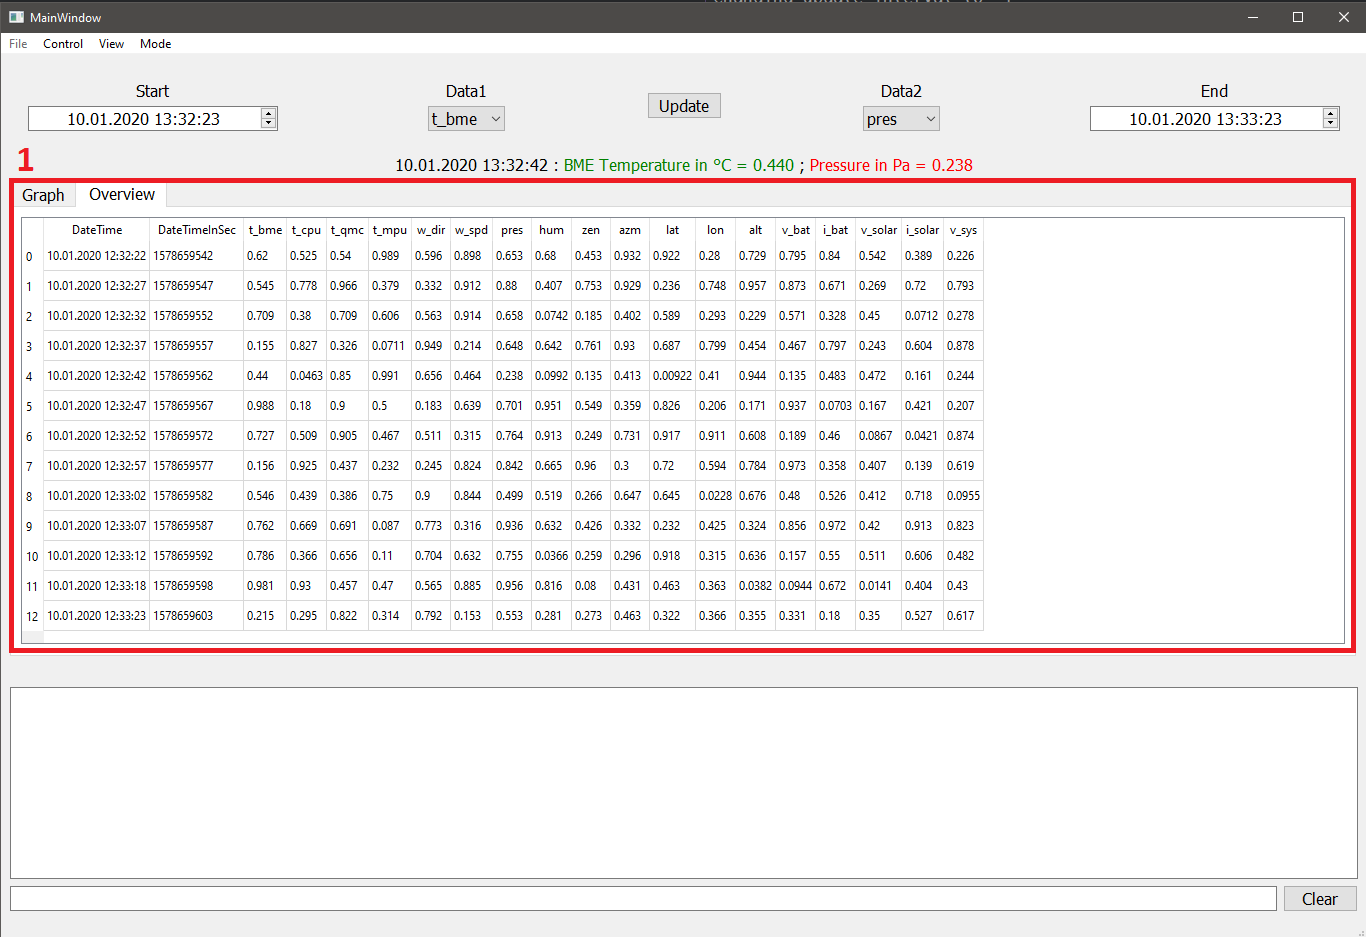
\includegraphics[width=\textwidth]{./img/ui_simulated_table}
\end{figure}
\end{frame}
\begin{frame}
  \frametitle{Geplante Funktionen}
  \begin{itemize}
  \item Speichern und Laden von Messdaten auf dem Computer
  \item Auslagerung der Kommunikation mit der Wetterstation in einen eigenen Task
  \item Einstellen der Kommunikationsschnittstelle über die Benutzeroberfläche
  \item Benutzerdefinierte Änderung der Position und des Datums / der Zeit über ein Bedienelement
  \end{itemize}
\end{frame}

\section{3D gedruckte Komponenten}
\begin{frame}
  \frametitle{Nebengehäuse}
  \begin{itemize}
  \item Sichere Unterbringung von GPS-Modul, Kompass-Modul, und Neigungssensor
  \item Befestigung an der Wetterstation mittels Schrauben
  \item Befestigung des Deckels mittels Steckverbindung und Kabelbindern
  \end{itemize}
  \begin{figure}[H]
    \centering 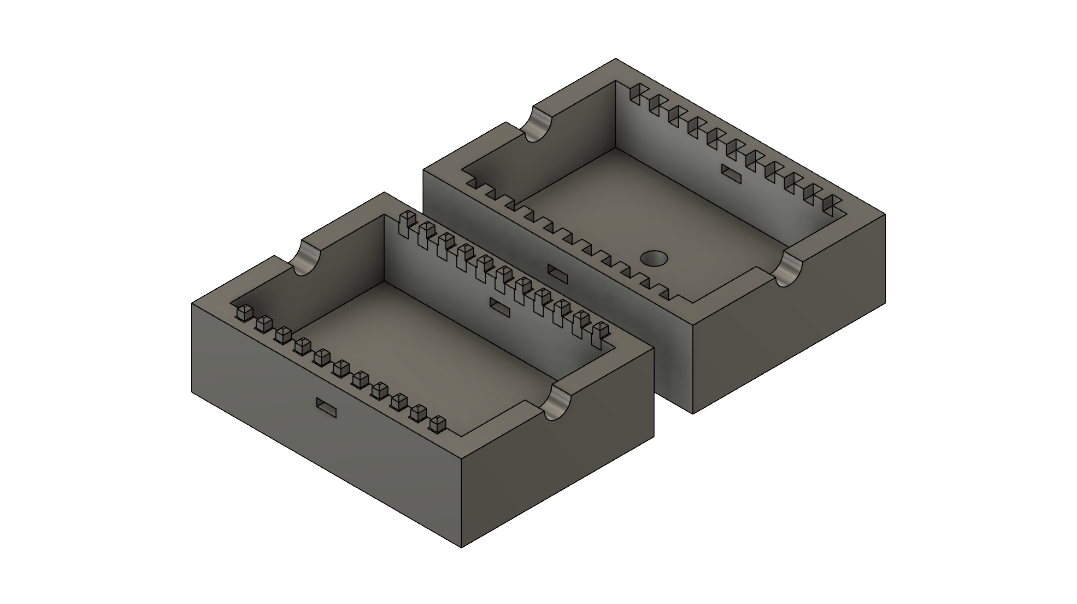
\includegraphics[width=.7\textwidth]{./img/ST_Halterv5}
  \end{figure}
\end{frame}
\begin{frame}
  \begin{itemize}
  \item Für die Verbindung des Masts (Anemometer und Windfahne) mit der Wetterstation
  \item Befestigung an de Wetterstation mittels Steckverbindung
  \item Verbindung mit dem Mast über Steckverbindung und optionale Schraubverbindung
  \end{itemize}
  \frametitle{Adapter}
  \begin{figure}[H]
    \centering 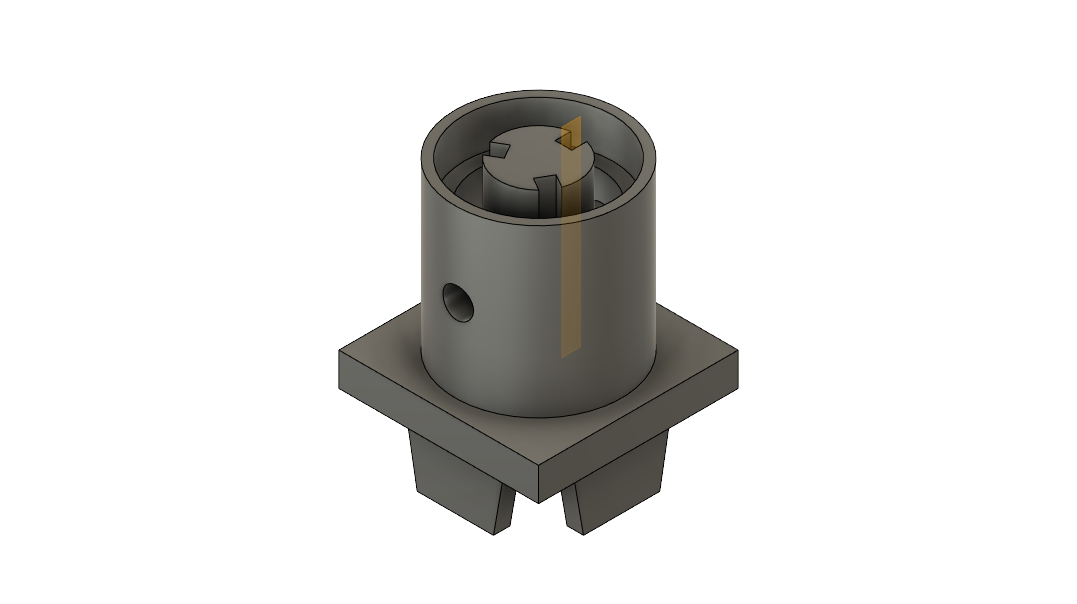
\includegraphics[width=.7\textwidth]{./img/ST_Adapterv4}
  \end{figure}
\end{frame}
\begin{frame}
  \frametitle{Hauptgehäuse}
  \begin{itemize}
  \item Für die Unterbringung des Mikrocontrollers, der Spannungsversorgung und des Motortreibers
  \item Befestigung an der Wetterstation mittels Klebverbindung
  \item Befestigung des Deckels mittels Steckverbindung und optionalen Kabelbindern
  \end{itemize}
  \begin{figure}[H]
    \centering
    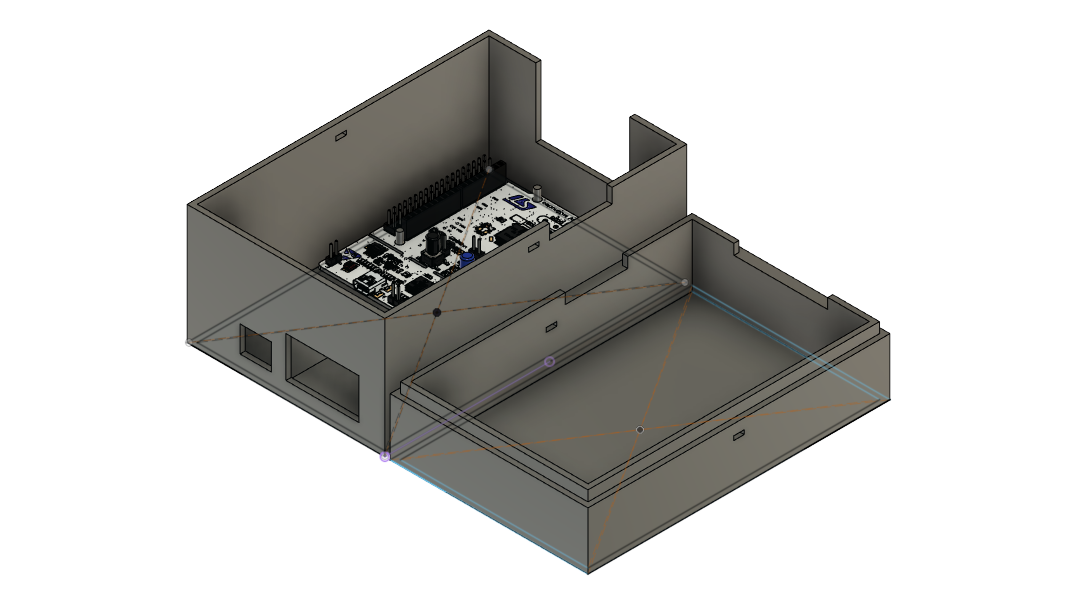
\includegraphics[width=.7\textwidth]{./img/ST_MainBodyv13}
  \end{figure}
\end{frame}


\section{Spannungsversorgung}
\begin{frame}
\frametitle{Grundlegendes}
\begin{itemize}
\item Erstellung von zwei Platinen (Power- und Sensorboard)
\item Steckbarer Aufbau
\item Entwurf mit Altium Circuit Maker
\end{itemize}

\end{frame}
\begin{frame}
  \frametitle{Power-Board}
  \begin{figure}[H]
    \centering
    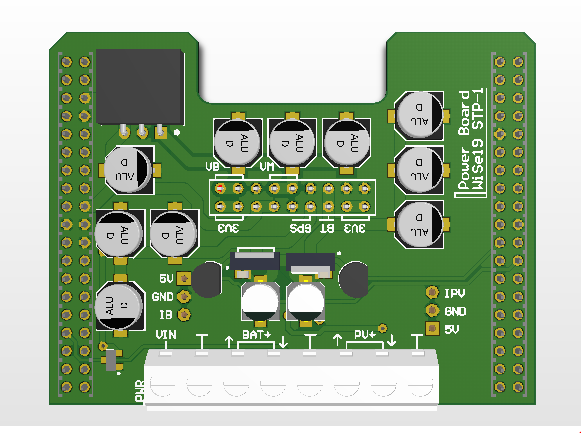
\includegraphics[width=0.7\textwidth]{./img/PCB_Power_3D_top.PNG}
  \end{figure}
\end{frame}

\begin{frame}
  \frametitle{Power-Board}
	\begin{itemize}
		\item Erzeugung von 5V
		\item Messung von Strom und Spannung
		\item Energiesparmaßnahmen
	\end{itemize}

\end{frame}

\begin{frame}
	\frametitle{Spannungsabschaltung 5V}
	 \begin{figure}[H]
    		\centering
   		 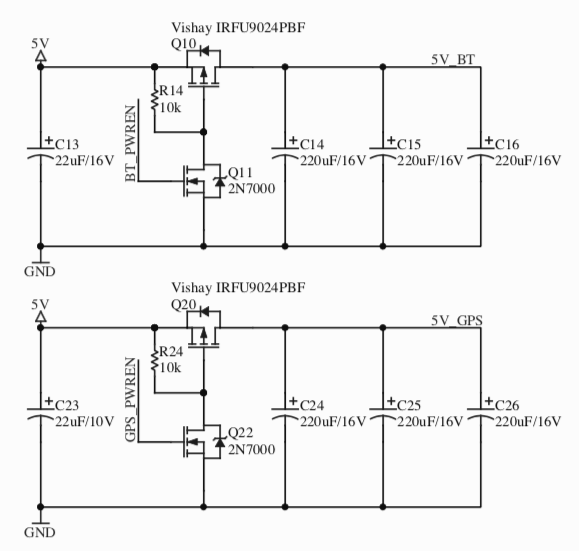
\includegraphics[width=0.7\textwidth]{./img/spannungsabschaltung.png}
 	 \end{figure}

\end{frame}


\begin{frame}
	\frametitle{Sensor-Board}
	 \begin{figure}[H]
    		\centering
    		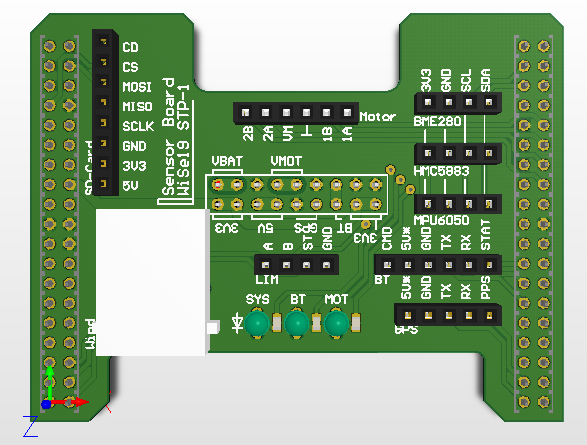
\includegraphics[width=0.7\textwidth]{./img/PCB_Sensors_3D_top.PNG}
  	 \end{figure}
\end{frame}


\section{Fazit}
\begin{frame}
	\frametitle{Wetterstation}
	 \begin{figure}[H]
    		\centering
    		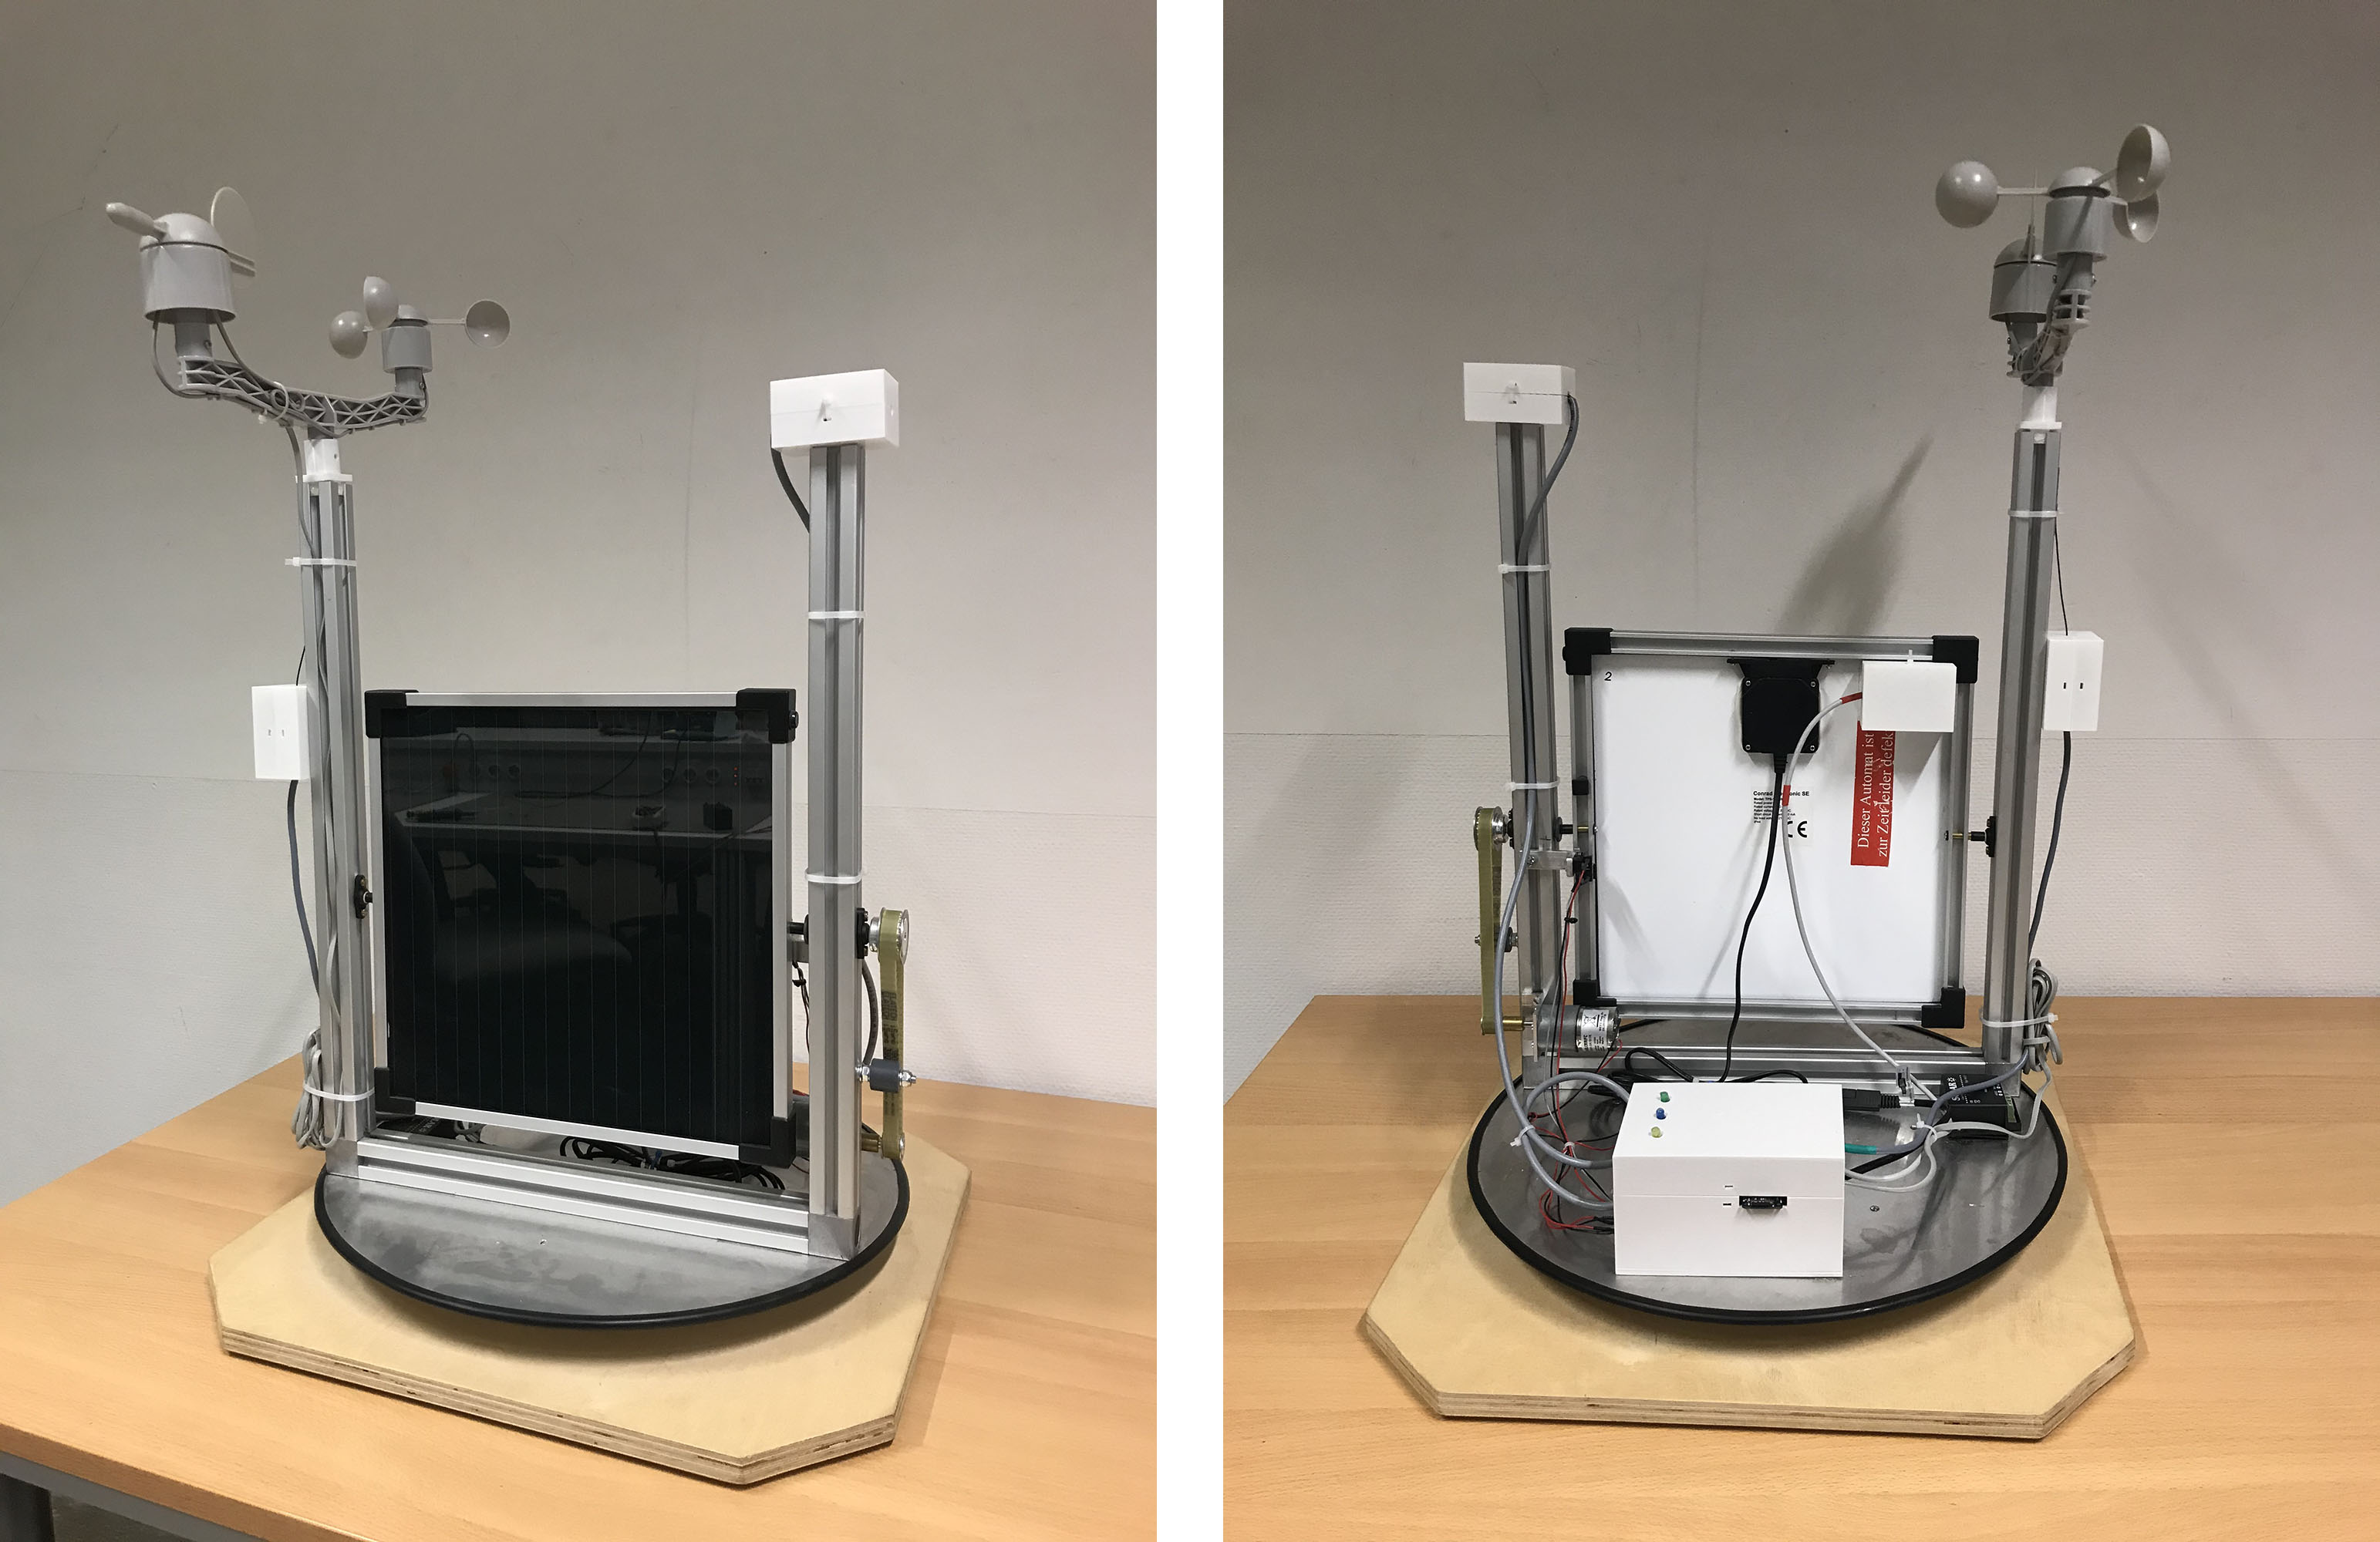
\includegraphics[width=0.7\textwidth]{./img/Wetterstaion_fertig1.JPG}
  	 \end{figure}
\end{frame}

\begin{frame}
	\frametitle{Fazit}
	\begin{itemize}
		\item Projektanforderungen erfüllt
		\item Erweiterung um GUI
		\item Wasserfestigkeit nicht gegeben
		\item Verbesserungsmöglichkeiten Panelaufhängung
	\end{itemize}

\end{frame}



% ----------------------------------------------------------------------------------------
% PRESENTATION SLIDES OLD
% ----------------------------------------------------------------------------------------

% \section{Software}
% % - zusammenfassen der Puntke aus Vorlage - eingrenzung Messbereiche
% \subsection{Fertig}
% \begin{frame}
%   \frametitle{Software - Fertig}
%   \begin{itemize}
%   \item \emph{Grundgerüst}
%   \item \emph{Ansteuerung I2C, SPI, UART, ADC, RTC}
%   \item \emph{Einlesen und Umrechnen der Sensordaten}
%   \item \emph{Lageregelung}
%   \item \emph{Auswertung NMEA-Sentences vom GPS-Modul}
%   \item \emph{Berechnung von Azimut und Elevation}
%   \item \emph{Kommunikation ÃŒber Bluetooth}
%   \item \emph{Externe Bibliothek für FAT32-Dateisystem}
%   \item \emph{Energiesparmaßnahmen}
%   \end{itemize}
% \end{frame}

% \begin{frame}
%   \frametitle{Berechnung der Sonnenposition}
%   \begin{itemize}
%   \item Berechnung von Zenith und Azimut
%   \item Implementierung nach \citet[]{Roderick1992}
%   \end{itemize}
%   \begin{figure}[hbtp]
%     \centering
%     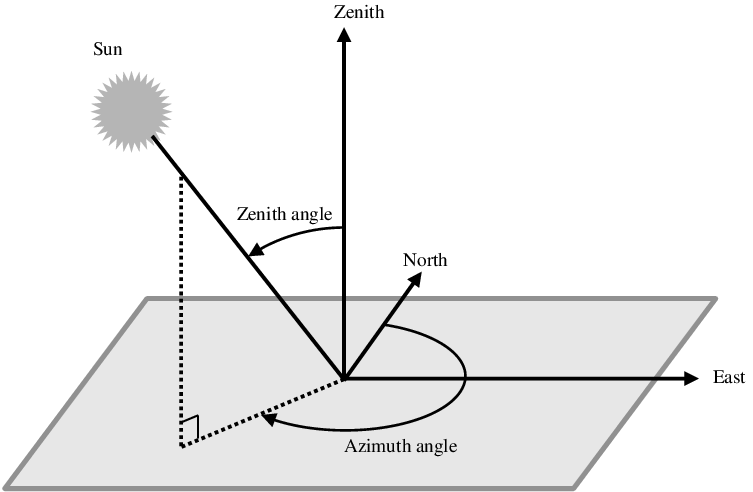
\includegraphics[width=0.6\textwidth]{./img/Representation-of-azimuth-and-zenith-angles.png}
%     \caption{Beschreibung der Sonnenposition durch Zenith und
%     Azimut~\cite[]{Nou2016}}\label{fig:zen_azi}
%   \end{figure}
% \end{frame}
% \begin{frame}
%   \frametitle{Berechnung der Sonnenposition (Beispiel)}
%   \begin{itemize}
%   \item Hamburg, 26.11.2019, 9:30h
%   \item Zenith = 81.1°
%   \item Azimuth = 143.3°
%   \end{itemize}
%   \begin{figure}[hbtp]
%     \centering
%     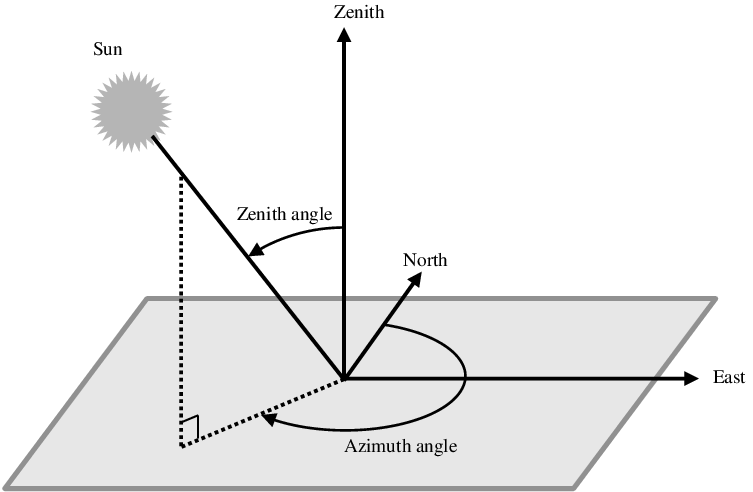
\includegraphics[width=0.6\textwidth]{./img/Representation-of-azimuth-and-zenith-angles.png}
%     \caption{Beschreibung der Sonnenposition durch Zenith und
%     Azimut~\cite[]{Nou2016}}\label{fig:zen_azi}
%   \end{figure}
% \end{frame}
% \subsection{Ausstehend}
% \begin{frame}
%   \frametitle{Software - Ausstehend}
%   \begin{itemize}
%   \item \emph{Zeitgesteuerte Nachführung des Panels}
%   \item \emph{Bluetooth: AT command set; Demo-Mode}
%   \item \emph{Visualisierungssoftware auf einem PC}
%   \item \emph{Speichern der Sensordaten auf der SD-Karte}
%   \end{itemize}
% \end{frame}

% % \end{frame}
% \section{Elektronik}
% % - Sensoren kurz vorstellen und Bezug auf Anforderungen nehmen
% \begin{frame}
%   \frametitle{Elektronik - Fertig}
%   \subsection{Fertig}
        
%   \begin{itemize}
%   \item \emph{Spannungsversorgung}
%   \item \emph{Schaltplan}
%   \item \emph{Platinenlayout}
%   \item \emph{Test der Motoren}
%   \end{itemize}
% \end{frame}

% \begin{frame}
%   \frametitle{Elektronik - Ausstehend}
%   \subsection{Ausstehend}
%   \begin{itemize}
%   \item \emph{Aufbau der Platine}
%   \item \emph{Verkabelung der Sensoren}
%   \item \emph{Kabelmanagement}
%   \end{itemize}
% \end{frame}
    
% \section{Aufbau}
% \begin{frame}
%   \frametitle{Aufbaue - Fertig}
%   \subsection{Fertig}
%   \begin{itemize}
%   \item \emph{Planung}
%   \item \emph{Stabilität des Solarmoduls}
%   \item \emph{3D-Druck - Halterung für Sensoren}
%   \end{itemize}
%   \begin{figure}[hbtp]
%     \centering
%     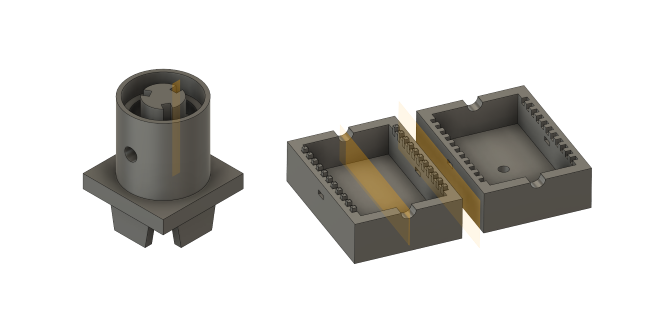
\includegraphics[width=0.8\textwidth]{./img/druck.png}
%     \caption{Adapter und Halter für die Sensoren}
%   \end{figure}
% \end{frame}

% \begin{frame}
%   \frametitle{Aufbau - Ausstehend}
%   \subsection{Ausstehend}
%   \begin{itemize}
%   \item \emph{Montage - Halterungen}
%   \item \emph{Montage - Sensoren}
%   \item \emph{Montage - Kabel}
%   \item \emph{Montage - Gehäuse (Platine)}
%   \item \emph{Montage - Spannungsversorgung}
%   \item \emph{3D-Druck - Gehäuse}
%   \end{itemize}
% \end{frame}

% \section{Zeitplan}
% % - groben Zeitplan vorstellen (Diagramm)

% \begin{frame}
%   \frametitle{Zeitplan}
%   \begin{itemize}
%   \item \emph{Planung ist vollständig abgeschlossen}
%   \item \emph{Fortführung nach Ankunft der Platine}
%   \item \emph{Dokumentation} %wird Montag eingereicht
%   \end{itemize}
% \end{frame}
\begin{frame}[allowframebreaks]
  \frametitle{Literatur- und Quellenverzeichnis}
  \bibliographystyle{plainnat} \bibliography{literature}
\end{frame}

\appendix
\section{Magnetometer-Kalibrierung}
\begin{frame}{Firmware}{Magnetometer-Kalibrierung}
    \begin{itemize}
        \item Bedingt durch Berechnung des Winkels über
    \end{itemize}
    \begin{equation*}
        \theta = 180\,^\circ + \mathrm{atan2}(x,\,y) \cdot \frac{180\,^\circ}{\pi}
    \end{equation*}
    \begin{itemize}
        \item Für korrekte Winkelbestimmung: Punkte aus X- und Y-Feldstärke kreisförmig um $(0,\,0)$
    \end{itemize}
    \begin{figure}[H]
        \centering
        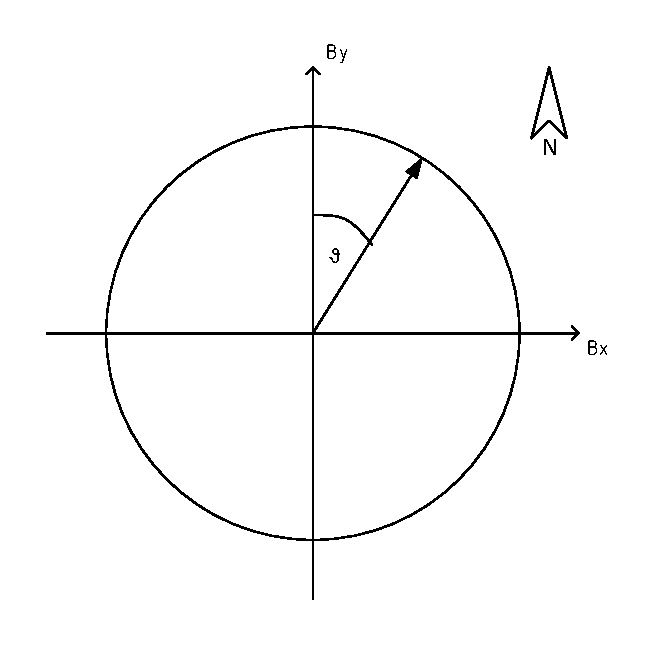
\includegraphics[width=.5\textwidth]{./img/Kursber.pdf}
    \end{figure}
\end{frame}

\begin{frame}{Firmware}{Magnetometer-Kalibrierung}
    \begin{itemize}
        \item Drehung des Turms um $360\,^\circ$
        \item Aufzeichnung Minimal-, Maximal- und Mittelwerte der X- und Y-Komponenten des Magnetfeldes
    \end{itemize}
    \begin{figure}[H]
        \centering
        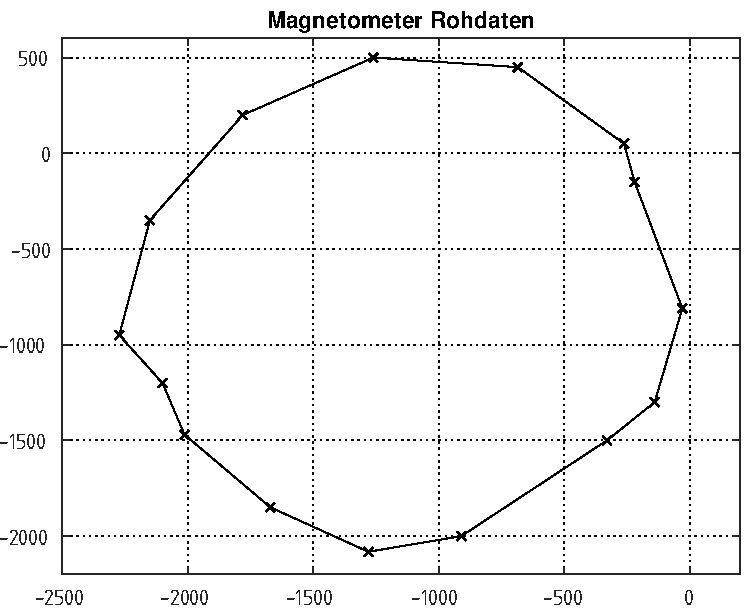
\includegraphics[width=.6\textwidth]{./img/qmc5883_raw.pdf}
    \end{figure}
    \begin{itemize}
        \item Kursberechnung liefert hier falsche Werte
    \end{itemize}
\end{frame}

\begin{frame}{Firmware}{Magnetometer-Kalibrierung}
    \begin{itemize}
        \item Mittelwerte: $(0,\,0)$ in den Mittelpunkt der Ellipse
        \item Min- und Max-Werte: Ellipse kreisförmig stauchen
    \end{itemize}
    \begin{figure}[H]
        \centering
        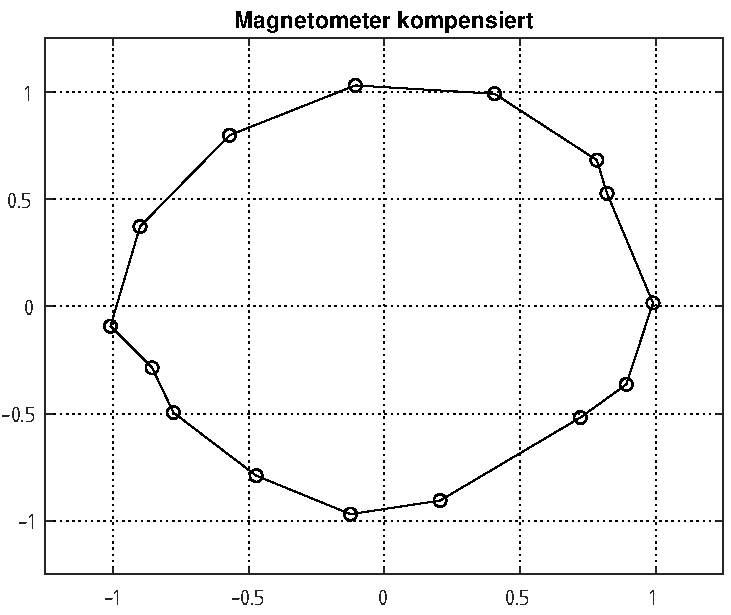
\includegraphics[width=.6\textwidth]{./img/qmc5883_compensated.pdf}
    \end{figure}
    \begin{itemize}
        \item Sensor für den aktuellen Standpunkt kalibriert
    \end{itemize}
\end{frame}

\section{AT-Befehlssatz}
\begin{frame}{Firwmare}{AT-Befehle}
    Konfiguration der Wetterstation über ``AT-Befehle'':
    \begin{itemize}
        \item AT+CTEMP: Temperaturmesswerte
        \item AT+CWIND: Windrichtung und -geschwindigkeit
        \item ...
        \item AT+CTURN=C: Magnetometer-Kalibrierung starten
        \item AT+CTRACK=1: Nachführung aktivieren
    \end{itemize}
\end{frame}

\begin{frame}{Firmware}{AT-Befehle}
    Für das Debugging:
    \begin{itemize}
        \item AT+CDEBUG: Debug-Ausgabe auf Bluetooth umleiten
        \item AT+CGNSTST: NMEA 0183 auf Bluetooth umleiten
    \end{itemize}
    \begin{figure}[H]
        \centering
        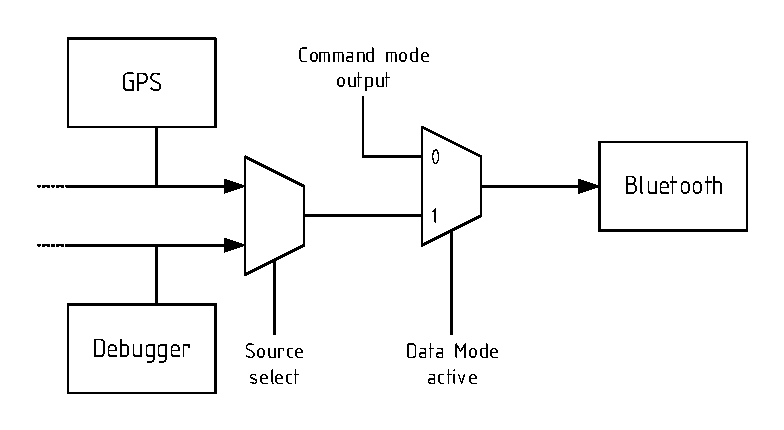
\includegraphics[width=.8\textwidth]{./img/Datenpfad_BT.pdf}
    \end{figure}
    \begin{itemize}
        \item Verlassen über `+++' 
    \end{itemize}
\end{frame}

\section{Benutzeroberfläche}
\begin{frame}
  \frametitle{Model-View-Controller}
  \begin{figure}[H]
    \centering 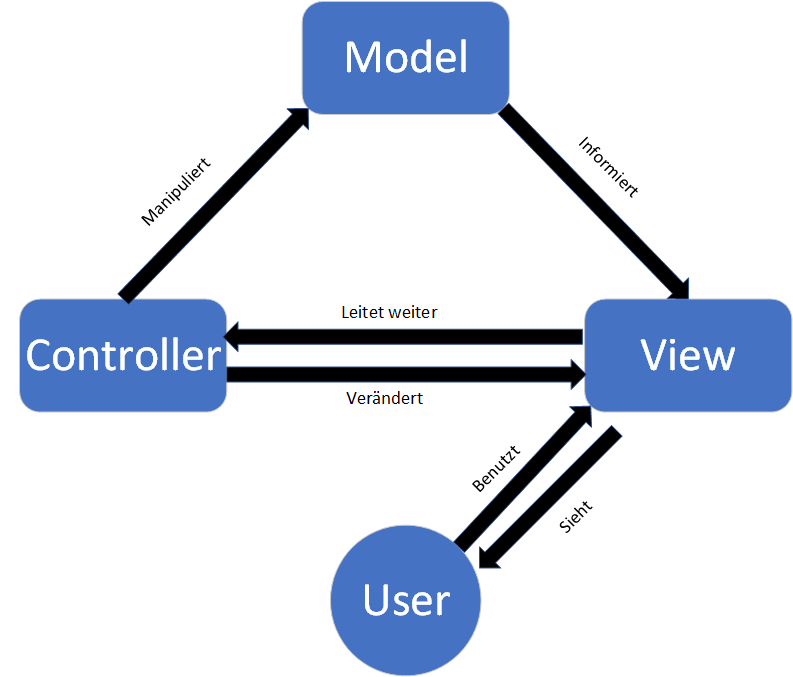
\includegraphics[width=.7\textwidth]{./img/MVC.png}
  \end{figure}
\end{frame}

\begin{frame}
  \frametitle{Verwendete Python-Packages}
  \begin{itemize}
  \item PyQt5: Als Framework für die Oberfläche.
  \item pyqtgraph: Für die graphische Darstellung der Messdaten.
  \item serial: Für die serielle Kommunikation, über Bluetooth, mit
    der Wetterstation.
  \item pandas: Für die Strukturierung der Messdaten.
  \item numpy: Für das Erstellen von Testdaten.
  \end{itemize}

\end{frame}

\begin{frame}
  \frametitle{Informationen zum 3D-Druck}
  \begin{itemize}
  \item Entwurf der Komponenten in Autocad Fusion 360
  \item Material der Komponenten: PLA
  \item Druck mit 2-3 Außenlagen und 10\%-20\% Infill
  \end{itemize}
\begin{figure}[H]
  \centering
  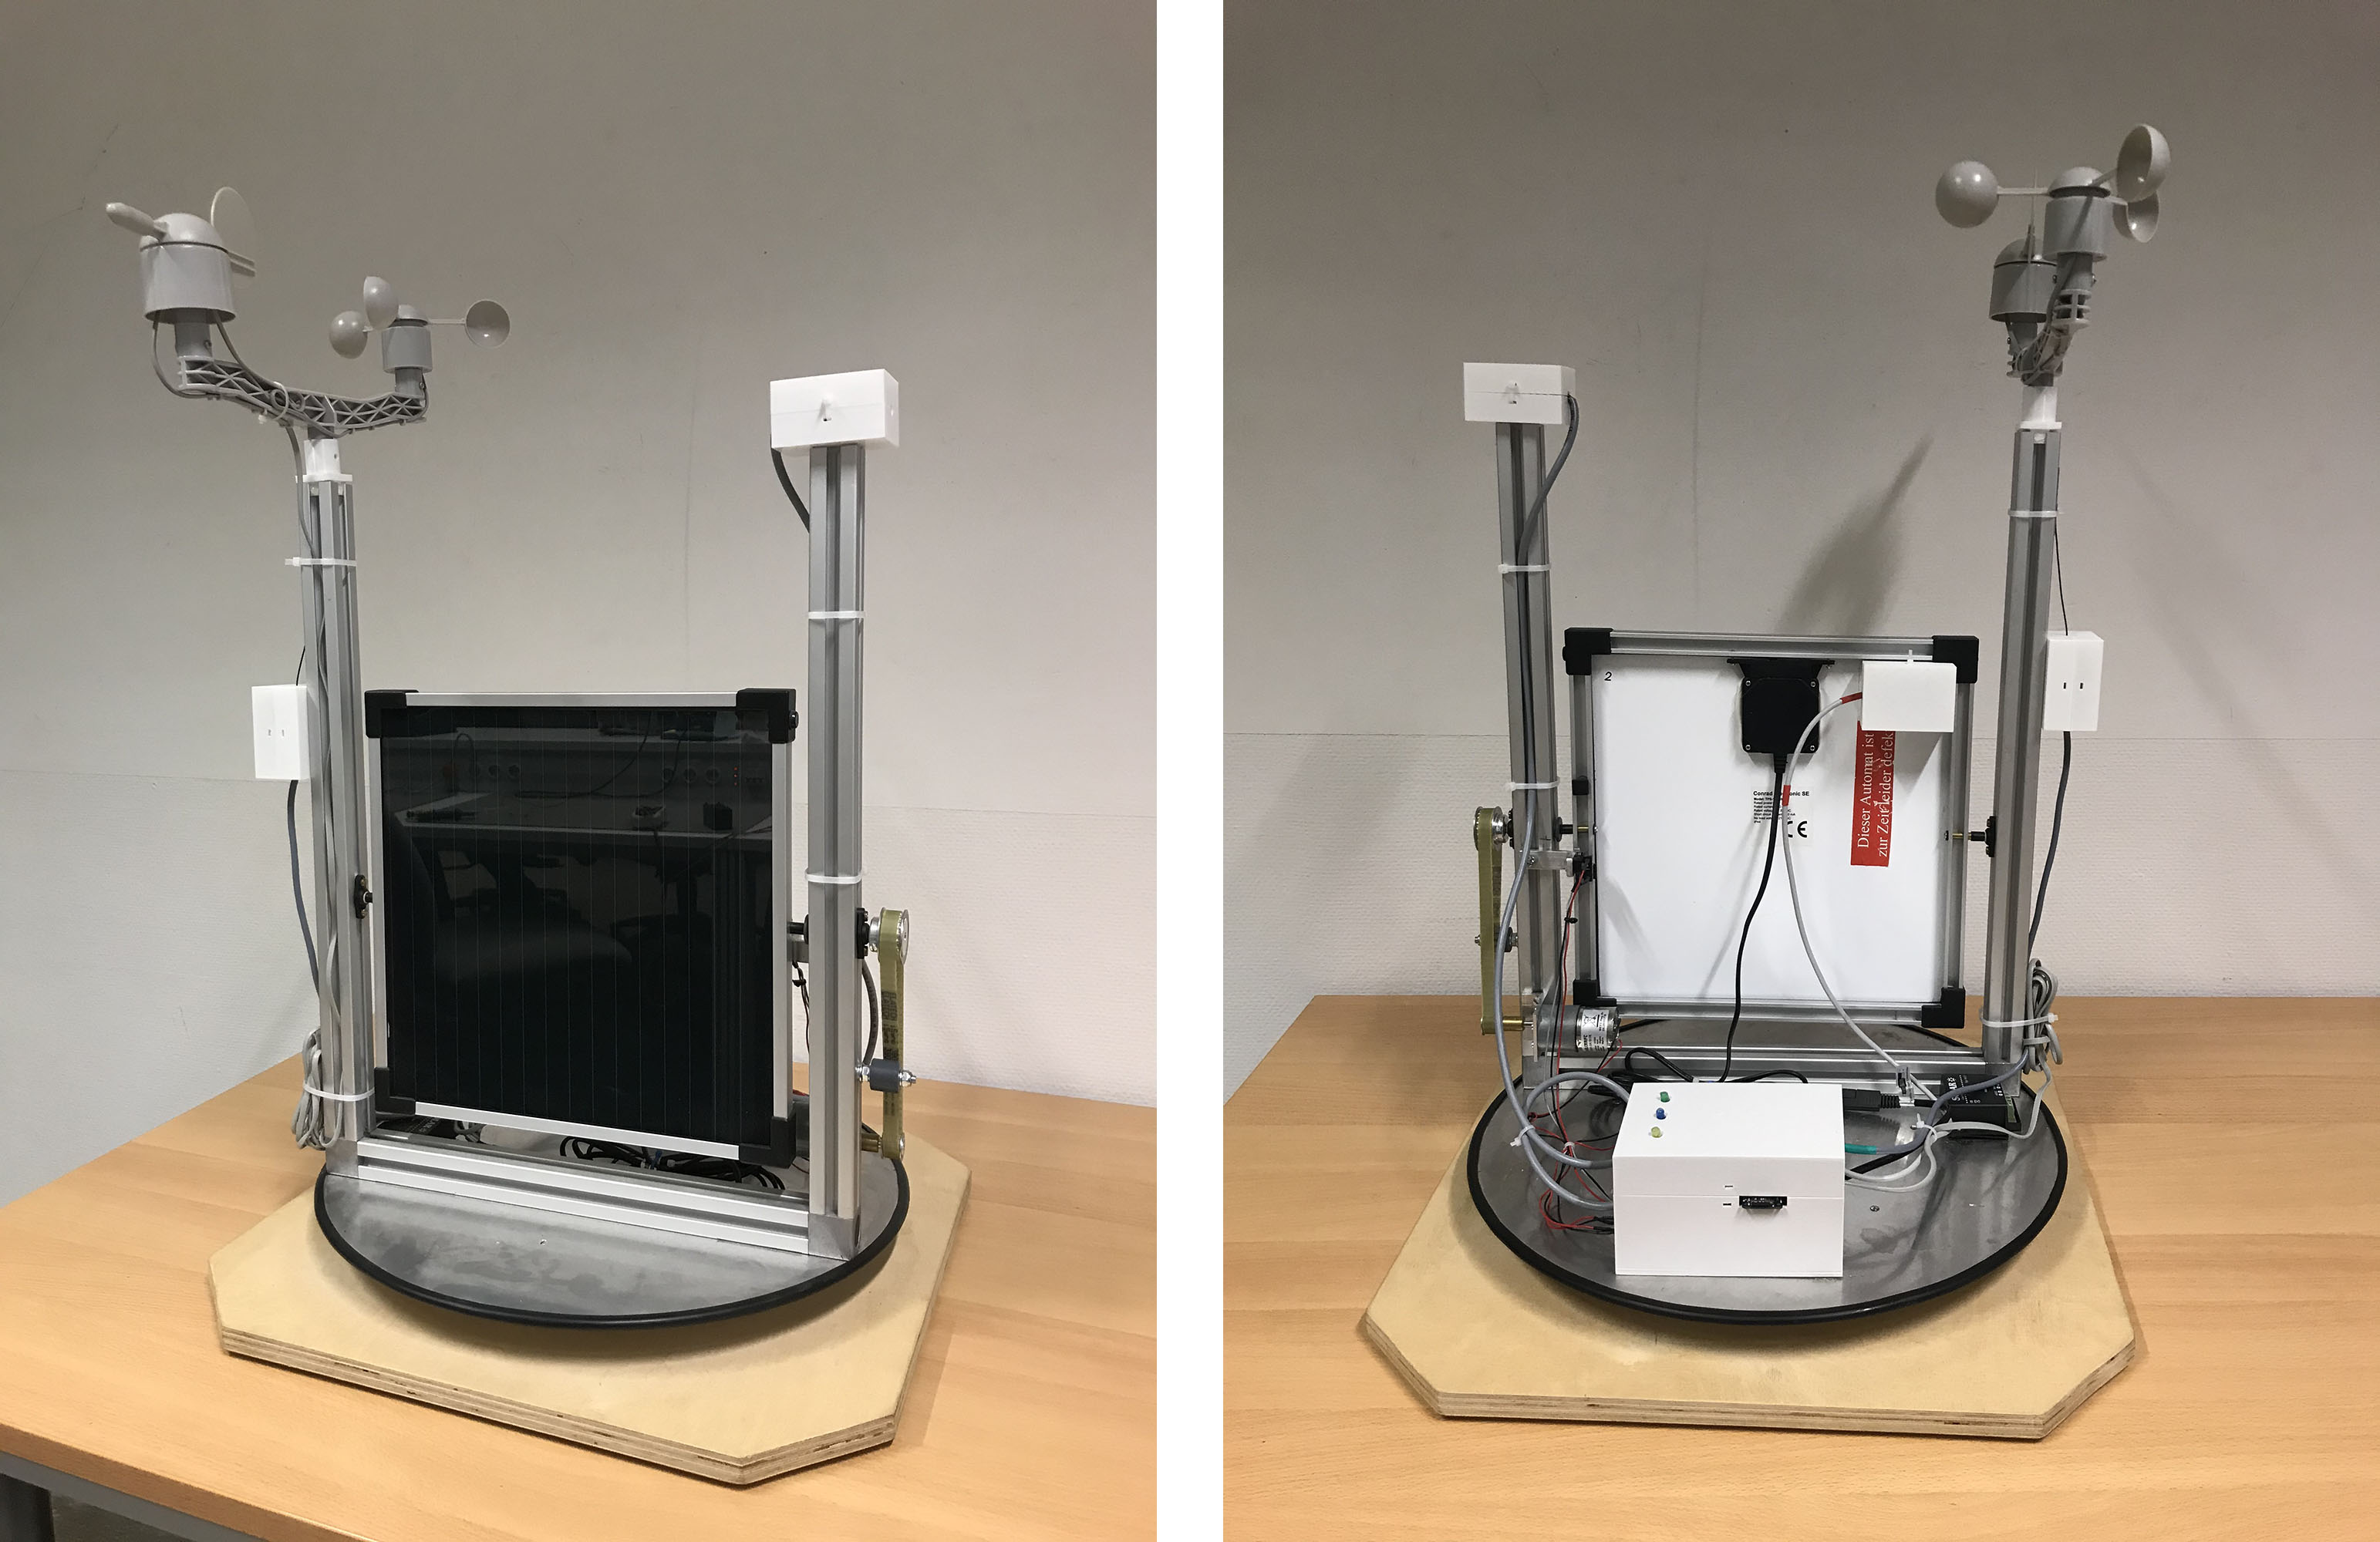
\includegraphics[width=0.7\textwidth]{./img/Wetterstaion_fertig1.jpg}
\end{figure}
  
\end{frame}

% ------------------------------------------------
% ----------------------------------------------------------------------------------------

\end{document}
%%% Local Variables:
%%% mode: latex
%%% TeX-master: t
%%% End:
